\documentclass[UTF8]{article}
\usepackage{graphicx}
\usepackage{subfigure}
\usepackage{amsmath}
\usepackage{makecell}
\usepackage[utf8]{inputenc}
\usepackage[space]{ctex} %中文包
\usepackage{listings} %放代码
\usepackage{xcolor} %代码着色宏包
\usepackage{CJK} %显示中文宏包
\usepackage{float}
\usepackage{diagbox}
\usepackage{bm}
\usepackage{ulem} 
\usepackage{amssymb}
\usepackage{soul}
\usepackage{color}
\usepackage{geometry}
\usepackage{fancybox} %花里胡哨的盒子
\usepackage{xhfill} %填充包, 可画分割线 https://www.latexstudio.net/archives/8245
\usepackage{multicol} %多栏包
\usepackage{enumerate} %可以方便地自定义枚举标题
\usepackage{enumitem}
\usepackage{multirow} %表格中多行单元格合并
\usepackage{wasysym} %可以使用wasysym里的一堆奇奇怪怪的符号
\usepackage{hyperref} % url
%%%%%%%%%%%%%%%伪代码%%%%%%%%%%%%%%%
\usepackage{amsmath}
\usepackage{algorithm}
\usepackage{algorithmicx}
\usepackage[noend]{algpseudocode}
%%%%%%%%%%%%%%%画图包%%%%%%%%%%%%%%%
\usepackage{tikz}
\usepackage{pgfplots} % http://pgfplots.sourceforge.net/gallery.html
\usetikzlibrary{pgfplots.patchplots} % 拟合支持
\usetikzlibrary{arrows,shapes,automata,petri,positioning,calc} % 状态图支持
\usetikzlibrary{arrows.meta} % 箭头
\usetikzlibrary{shadows} % 阴影支持
\usepackage{forest} % 画树

\geometry{left = 1.5cm, right = 1.5cm, top=1.5cm, bottom=2cm}

\definecolor{mygreen}{rgb}{0,0.6,0}
\definecolor{mygray}{rgb}{0.5,0.5,0.5}
\definecolor{mymauve}{rgb}{0.58,0,0.82}
\lstset{
	backgroundcolor=\color{white}, 
	%\tiny < \scriptsize < \footnotesize < \small < \normalsize < \large < \Large < \LARGE < \huge < \Huge
	basicstyle = \footnotesize,       
	breakatwhitespace = false,        
	breaklines = true,                 
	captionpos = b,                    
	commentstyle = \color{mygreen}\bfseries,
	extendedchars = false,
	frame = shadowbox, 
	framerule=0.5pt,
	keepspaces=true,
	keywordstyle=\color{blue}\bfseries, % keyword style
	language = C++,                     % the language of code
	otherkeywords={string}, 
	numbers=left, 
	numbersep=5pt,
	numberstyle=\tiny\color{mygray},
	rulecolor=\color{black},         
	showspaces=false,  
	showstringspaces=false, 
	showtabs=false,    
	stepnumber=1,         
	stringstyle=\color{mymauve},        % string literal style
	tabsize=4,          
	title=\lstname           
}

%\sum\nolimits_{j=1}^{M}   上下标位于求和符号的水平右端,
%\sum\limits_{j=1}^{M}   上下标位于求和符号的上下处,
%\sum_{j=1}^{M}  对上下标位置没有设定,会随公式所处环境自动调整。

%%%%%%%%%%%%%画图包%%%%%%%%%%%%%
\usepackage{tikz}
%%%%%%%%%%%%%好看的矩形%%%%%%%%%%%%%
\tikzset{
	rect1/.style = {
		shape = rectangle,% 指定样式
		minimum height=2cm,% 最小高度
		minimum width=4cm,% 最小宽度
		align = center,% 文字居中
		drop shadow,% 阴影
	}
}
%%%%%%%%%%%%%画图背景包%%%%%%%%%%%%%
\usetikzlibrary{backgrounds}

%%%%%%%%%%%%%在tikz中画一个顶点%%%%%%%%%%%%%
%%%%%%%%%%%%%#1:node名称%%%%%%%%%%%%%
%%%%%%%%%%%%%#2:位置%%%%%%%%%%%%%
%%%%%%%%%%%%%#3:标签%%%%%%%%%%%%%
\newcommand{\newVertex}[3]{\node[circle, draw=black, line width=1pt, scale=0.8] (#1) at #2{#3}}
%%%%%%%%%%%%%在tikz中画一条边%%%%%%%%%%%%%
\newcommand{\newEdge}[2]{\draw [black,very thick](#1)--(#2)}
%%%%%%%%%%%%%在tikz中放一个标签%%%%%%%%%%%%%
%%%%%%%%%%%%%#1:名称%%%%%%%%%%%%%
%%%%%%%%%%%%%#2:位置%%%%%%%%%%%%%
%%%%%%%%%%%%%#3:标签内容%%%%%%%%%%%%%
\newcommand{\newLabel}[3]{\node[line width=1pt] (#1) at #2{#3}}

%%%%%%%%%%%%%强制跳过一行%%%%%%%%%%%%%
\newcommand{\jumpLine} {\hspace*{\fill} \par}
%%%%%%%%%%%%%关键点指令,可用itemise替代%%%%%%%%%%%%%
\newcommand{\keypoint}[2]{$\bullet$\textbf{#1}\quad#2\par}
%%%%%%%%%%%%%<T>平均值表示%%%%%%%%%%%%%
\newcommand{\average}[1]{\left\langle #1\right\rangle }
%%%%%%%%%%%%%表格内嵌套表格%%%%%%%%%%%%%
\newcommand{\tabincell}[2]{\begin{tabular}{@{}#1@{}}#2\end{tabular}}
%%%%%%%%%%%%%大黑点item头%%%%%%%%%%%%%
\newcommand{\itemblt}{\item[$\bullet$]}
%%%%%%%%%%%%%大圈item头%%%%%%%%%%%%%
\newcommand{\itemc}{\item[$\circ$]}
%%%%%%%%%%%%%大星星item头%%%%%%%%%%%%%
\newcommand{\itembs}{\item[$\bigstar$]}
%%%%%%%%%%%%%右▷item头%%%%%%%%%%%%%
\newcommand{\itemrhd}{\item[$\rhd$]}
%%%%%%%%%%%%%定义为%%%%%%%%%%%%%
\newcommand{\defas}{=_{df}}
%%%%%%%%%%%%%偏导%%%%%%%%%%%%%
\newcommand{\partialx}[2]{\frac{\partial #1}{\partial #2}}
%%%%%%%%%%%%%蕴含%%%%%%%%%%%%%
\newcommand{\imp}{\rightarrow}
%%%%%%%%%%%%%上取整%%%%%%%%%%%%%
\newcommand{\ceil}[1]{\lceil#1\rceil}
%%%%%%%%%%%%%下取整%%%%%%%%%%%%%
\newcommand{\floor}[1]{\lfloor#1\rfloor}

%%%%%%%%%%%%%双线分割线%%%%%%%%%%%%%
\newcommand*{\doublerule}{\hrule width \hsize height 1pt \kern 0.5mm \hrule width \hsize height 2pt}
%%%%%%%%%%%%%双线中间可加东西的分割线%%%%%%%%%%%%%
\newcommand\doublerulefill{\leavevmode\leaders\vbox{\hrule width .1pt\kern1pt\hrule}\hfill\kern0pt }
%%%%%%%%%%%%%左大括号%%%%%%%%%%%%%
\newcommand{\leftbig}[1]{\left\{\begin{array}{l}#1\end{array}\right.}
%%%%%%%%%%%%%矩阵%%%%%%%%%%%%%
\newcommand{\mat}[2]{\left[\begin{array}{#1}#2\end{array}\right]}
%%%%%%%%%%%%%组合%%%%%%%%%%%%%
\newcommand{\comb}[2]{\left(\begin{array}{c}#1 \\ #2\end{array}\right)}
%%%%%%%%%%%%%可换行圆角文本框%%%%%%%%%%%%%
\newcommand{\ovalboxn}[1]{\ovalbox{\tabincell{l}{#1}}}
%%%%%%%%%%%%%设置section的counter, 使从1开始%%%%%%%%%%%%%
\setcounter{section}{0}

%%%%%%%%%%%%%Colors%%%%%%%%%%%%%
\newcommand{\lightercolor}[3]{% Reference Color, Percentage, New Color Name
	\colorlet{#3}{#1!#2!white}
}
\newcommand{\darkercolor}[3]{% Reference Color, Percentage, New Color Name
	\colorlet{#3}{#1!#2!black}
}
\definecolor{aquamarine}{rgb}{0.5, 1.0, 0.83}
\definecolor{Seashell}{RGB}{255, 245, 238} %背景色浅一点的
\definecolor{Firebrick4}{RGB}{255, 0, 0}%文字颜色红一点的
\lightercolor{gray}{20}{lgray}
\newcommand{\hlg}[1]{
	\begingroup
	\sethlcolor{lgray}%背景色
	\textcolor{black}{\hl{\mbox{#1}}}%textcolor里面对应文字颜色
	\endgroup
}



\title{大数据算法 HW1}
\author{PB18111697 王章瀚}

\begin{document}
\maketitle
\section*{1.}
\noindent \textbf{假设 $\delta, \theta\in (0,1)$, 给定集合 $U$ 以及其一个子集 $V$, $|V|/|U|=a$}
\subsection*{(1).}
\noindent \textbf{如果我们从 $U$ 均匀采样本 $S$, 并确保 $S\cap V\not=\varnothing$ 的概率大于 $1-\delta$, $|S|$ 至少要多大?}
\jumpLine \noindent 
考虑有放回采样:
\begin{align*}
	P(S\cap V\not=\varnothing)&=1-P(S\cap V=\varnothing) \\
	&=1- \frac{|U|-|V|}{|U|}^{|S|} \\
	&=1-(1-a)^{|S|} \\
	&>1-\delta
\end{align*}
可知, $|S|$ 应当满足 $|S|>\log_{(1-a)}\delta$

\subsection*{(2).}
\noindent \textbf{如果我们要确保 $|S\cap V|\in (1\pm\theta)a|S|$ 的概率大于 $1-\delta$, $|S|$ 至少要多大?}
\jumpLine \noindent 
显然, 随机抽样在 $V$ 里的概率为 $a$, 可以考虑 $|S|$ 个独立同分布于 $B(1,a)$ 的随机变量 $X_1,\cdots,X_{|S|}$\\
即对 $i=1,\cdots,|S|$ 有
$$P(X_i=k)=\left\{\begin{array}{ll}a & ,k=1 \\ 1-a & ,k = 0\end{array}\right.$$
那么 $P(|S\cap V|=k)=P(\sum\limits_{i=1}^{|S|}X_i=k)$, 且 $E[|S\cap V|]=a|S|$ \\
由 Chernoff Bounds: 
\begin{align*}
	P(|S\cap V|\notin (1\pm\theta)a|S|)&=P(|S\cap V|\notin (1\pm\theta)E[|S\cap V|])\\
	&=P\left(\left|\sum\limits_{i=1}^{|S|}X_i\right|\notin a|S|\pm a\theta|S| \right) \\
	&\le 2\exp(-2|S|(a\theta)^2)
\end{align*}
即 $P(|S\cap V|\in (1\pm\theta)a|S|)>1-2\exp(-2|S|(a\theta)^2)$ \\
故要想$P(|S\cap V|\in (1\pm\theta)a|S|)>1-\delta$, 应确保
$$1-2\exp(-2|S|(a\theta)^2) > 1-\delta$$
即 $$|S|>\frac{\ln\frac{2}{\delta}}{2(a\theta)^2}$$


\section*{2.}
\noindent \textbf{给定高维空间 $R^d$ 的一个点集 $P$, $|P|=n$, 如果我们进行 k-means 聚类,(1). 能否通过 J-L 变换来降低复杂度? (2).能否通过 PCA 来降低复杂度? 请分别给出详细的理论分析. (比如, 如果我们有一个 $\lambda$ 倍近似比的 k-means 聚类算法 A, 其复杂度为 T(n,d), 那么我们用 A 对降维之后的数据运算, 并将得到的结果返回原有空间, 得到近似比是多少? 整个过程复杂度是多少?)}
不妨依据题目意思, 假设我们有一个 $\lambda$ 倍近似比的 k-means 算法, 复杂度为 $T(n, d)$.
\subsection*{(1).}
\noindent \textbf{能否通过 J-L 变换来降低复杂度?}
\jumpLine \noindent 
JL 变换的时间复杂度是 $O(nd\frac{\log n}{\epsilon^2})$, 能够保证的是降维到 $k=O(\frac{\log n}{\epsilon^2})$ 后, 仍有
$$(1-\epsilon)\|u-v\|^2\le\|f(u)-f(v)\|^2\le(1+\epsilon)\|u-v\|^2$$
即其降维后距离变化不会超过 $\epsilon$ 倍. \\
k-means 算法的复杂度是 $T(n,d)$, 近似比是 $\lambda$, 目标是
$$\mathrm{minimize} \sum\limits_{x\in X}\|\phi_S(x),x\|^2$$
因此降维之后, 相当于是
$$\mathrm{minimize} \sum\limits_{x\in X}\|\phi_S(f(x)),f(x)\|^2$$
且其中有
\textcolor{red}{
\begin{align*}
	C_{recover} &= \sum\limits_{l=1}^k\sum\limits_{x\in C'_i}\|x - C_l'\|^2 \\
	&=\sum\limits_{l=1}^k\sum\limits_{x_i, x_j\in C'_i} \frac{\|x_i-x_j\|^2}{2n_l} \\
	&\le \frac{1}{1-\epsilon}\sum\limits_{l=1}^k\sum\limits_{x_i, x_j\in C'_i} \frac{\|\phi(x_i)-\phi(x_j)\|^2}{2n_l} \\
	&\le \frac{\lambda}{1-\epsilon}\sum\limits_{l=1}^k\sum\limits_{x_i, x_j\in C'_i} \frac{\|\phi(x_i)-\phi(x_j)\|^2}{2n_l} \\
	&\le \lambda\frac{1+\epsilon}{1-\epsilon}\sum\limits_{l=1}^k\sum\limits_{x_i, x_j\in C'_i} \frac{\|\phi(x_i)-\phi(x_j)\|^2}{2n_l} \\
	&=\lambda\frac{1+\epsilon}{1-\epsilon} OPT
\end{align*}
}

由此可知, 近似比是 $\lambda(1+\epsilon)$.\\
相应时间复杂度包含如下几步:
\begin{itemize}
	\item JL 变换需要 $O(nd\frac{\log n}{\epsilon^2})$
	\item k-means 需要 $T(n,k)=T(n,\frac{\log n}{\epsilon^2})$
	\item JL 变换回去, 不考虑求逆矩阵的时间(JL正逆矩阵一般可以提前准备好, 与数据无关), 但逆变换依然需要一次矩阵乘法, 即 $O(nd\frac{\log n}{\epsilon^2})$
\end{itemize}
综上总共是 $O(2nd\frac{\log n}{\epsilon^2}) + T(n,\frac{\log n}{\epsilon^2})=O(nd\frac{\log n}{\epsilon^2}) + T(n,\frac{\log n}{\epsilon^2})$\\
因此, 只要能够保证 $nd\frac{\log n}{\epsilon ^2}=\omega (T(n,d))$, 就能够保证在 $\lambda(1+\epsilon)$ 近似比的条件下降低复杂度.

\subsection*{(2).}
\noindent \textbf{能否通过 PCA 来降低复杂度?}
\jumpLine \noindent 
对于 PCA 算法, 其复杂度包括 计算协方差矩阵 $O(d^2 n)$ 和 特征值分解 $O(d^3)$ 及正逆变换 $O(ndk)$, 故总共需要 $O(d^2n+d^3+ndk)$. 这里复杂度已经非常高, 并不太适合作为 k-means 算法的降维处理操作. \\
另一方面, PCA 算法没有一个近似比保证, 从这个角度来说, 它并不合适.

\textcolor{red}{
设 $P$ 已中心化, $C$ 为最优解对应的 center 集合, 其张成 $k-1$ 维子空间 $H$.
考虑经 $W\in \mathbb{R}^{(k-1)\times d}$ 将数据集 $P$ 投影到一个 $k-1$ 维超平面 $H'$ 上, 则 
$$\sum\limits_{i=1}^n\|p_i-\pi_{H'}(p_i)\|^2
\le
\sum\limits_{i=1}^n\|p_i-\pi_{H}(p_i)\|^2
\le
\sum\limits_{i=1}^n\|p_i-C(p_i)\|^2
$$
在 $P'$ $k-1$ 维空间上运行 k-means 算法, 得到 $C'(P')$ 为其center.
$\pi_{H'}(P_i)=W^T WP$
用三角不等式:
\begin{align*}
C_{recover}&=\sum\limits_{i=1}^n\|p_i-W^T C'(P_i)\|^2 \\
&\le \sum\limits_{i=1}^n\|p_i-\pi_{H'}(p_i)\|^2+\|\pi_{H'}(p_i) - W^T C'(p_i)\|^2\\
&=\sum\limits_{i=1}^n\|p_i-\pi_{H'}(p_i)\|^2 + \|W^T(Wp_i - C'(p_i))\|^2\\
\end{align*}
先估计这个:
\begin{align*}
\sum\limits_{i=1}^n\|Wp_i - C'(p_i)\|^2&\le \lambda \sum\limits_{i=1}^n\|Wp_i - WC(p_i)\|^2 \\
&=\lambda \sum\limits_{i=1}^n\|W(p_i - WC(p_i))\|^2 \\
&\le \lambda \sum\limits_{i=1}^n\|p_i-c(p_i)\|^2
\end{align*}
用这个可以放缩第二项, 最前面的不等式能放缩第一项.
}

\newpage
\section*{3.}
\noindent \textbf{请构造一个反例, 证明 Gonzalez 算法不能代替 k-means++ 算法用于 k-means 聚类的初始点选择.} 
\jumpLine \noindent 
如果用 Gonzalez 算法, 考虑一个二分类问题, 里面有四个点, 分别为狭长的矩形的四个顶点, 如下图:\\
\begin{center}
	\begin{tikzpicture} [scale=1.5] %将图放大
		%\draw[help lines] (-4,-4) grid (4,4);
		\draw[black][-] (-2,-0.2) -- (2,-0.2);
		\draw[black][-] (2,-0.2) -- (2,0.2);
		\draw[black][-] (2,0.2) -- (-2,0.2);
		\draw[black][-] (-2,0.2) -- (-2,-0.2);
		\node at (-2.1, -0.3) {A};
		\node at (2.1, -0.3) {B};
		\node at (2.1, 0.3) {C};
		\node at (-2.1, 0.3) {D};
	\end{tikzpicture}
\end{center}
由于随机性, 第一步可能选取的是 A, 然后类中心变成了矩形中心. 而后, 如果第二步选取的是 D, 那么就会导致分类结果是 \{A,B\}, \{C,D\}, 这明显和最优结果 \{A,D\},\{B,C\} 相差很多, 且无法被 k-means 迭代修正. \\
而如果使用 k-means++ 的办法, 则依然有一定概率(只是比较小)能够在第二步选择 B 或 C, 从而使得整个聚类达到最优.

\textcolor{red}{
应当用 (A)-[distance: x]-(B)-[distance:y]-(C) 的形式, 其中 $x \ll y$.
}

\section*{4.}
\noindent \textbf{请计算平面上以下 range 的 VC Dimension:}
\subsection*{(1). 矩形}
\noindent 考虑圆上 7 个点, (构成正七边形)
\begin{center}
\begin{minipage}{\linewidth/4}
\begin{figure}[H]
	\centering
	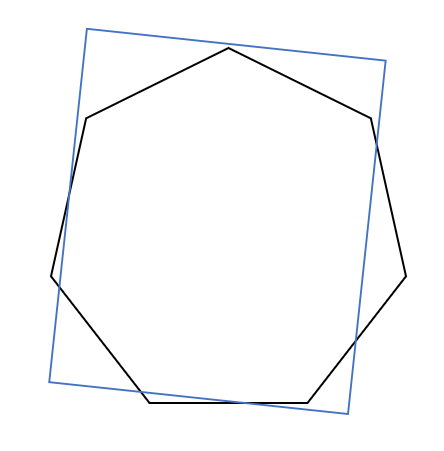
\includegraphics[width=\linewidth]{image/4.1.3.png}
	\caption{4.(1). 3 个点的比较不易想到的方法示意图}
\end{figure}
\end{minipage}
\begin{minipage}{\linewidth/4}
\begin{figure}[H]
	\centering
	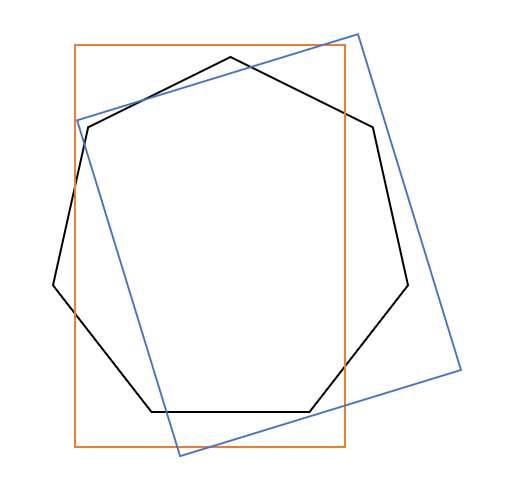
\includegraphics[width=\linewidth]{image/4.1.4.png}
	\caption{4.(1). 4 个点的比较不易想到的方法示意图}
\end{figure}
\end{minipage}
\begin{minipage}{\linewidth/4}
\begin{figure}[H]
	\centering
	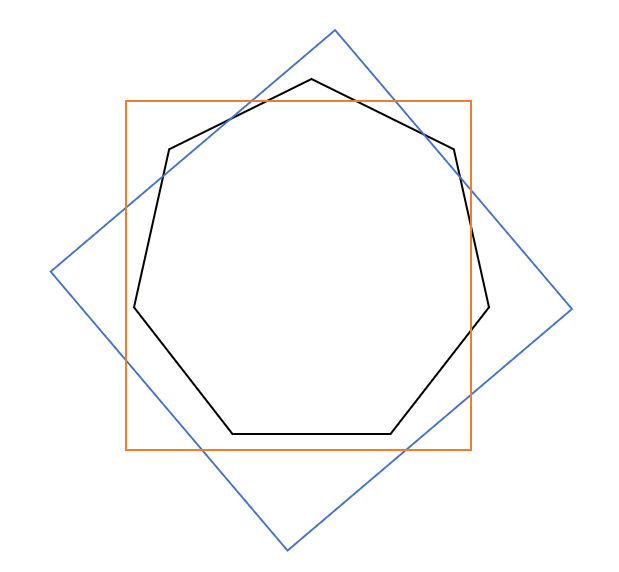
\includegraphics[width=\linewidth]{image/4.1.5.png}
	\caption{4.(1). 5 个点的比较不易想到的方法示意图}
\end{figure}
\end{minipage}
\end{center}
则显然其任意子集必然可以被某个矩形划分(子集大小为 1, 2, 6, 7 显然, 为 3, 4, 5 的不显然情况则如上所示(结合对称性)), 因此矩形的 VC-dimension 至少是 5. \\
而如果考虑正八边形, 由于有些边夹角已经小于90度, 直觉上难以画出可行解, 但我无法证明其不行.

\subsection*{(2). 半圆形}
\noindent 同样, 考虑前面矩形的那个五点情况, 一样可以得出半圆形在平面上的 VC-dimension 至少是 5. (即考虑子集大小为 1, 4, 5 均比较显然, 大小为 2 时, 比较不显然的情况在图中用绿线标出, 大小为 3 时, 所有(对称地)情况都用蓝色标出了)
\begin{center}
	\begin{figure}[H]
		\centering
		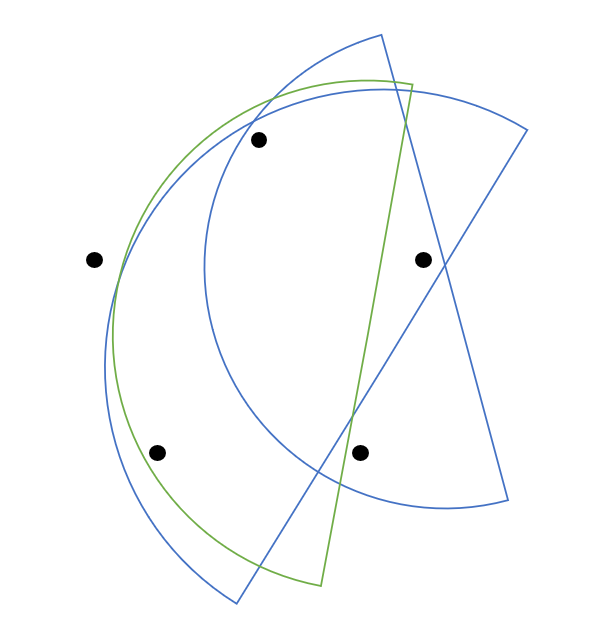
\includegraphics[width=\linewidth/3]{image/4.2.png}
		\caption{4.(2). 示意图}
	\end{figure}
\end{center}
如果能证明大于 5 不行, 那么半圆形的 VC 维就是 5.

\subsection*{(3). 凸多边形}
\noindent 显然, 凸多边形的 VC dimension 是无穷大的. 我们只需要考虑圆上均匀分割的 n 个点, 那么其中任意几个点构成的点集都可以用一个比由这些点构成的凸多边形包围. 且这里的 n 可以无限大.\\
因此, 凸多边形的 VC dimension 是 $\infty$ 的.

\end{document}



